


\tikzset{every picture/.style={line width=0.75pt}} %set default line width to 0.75pt        

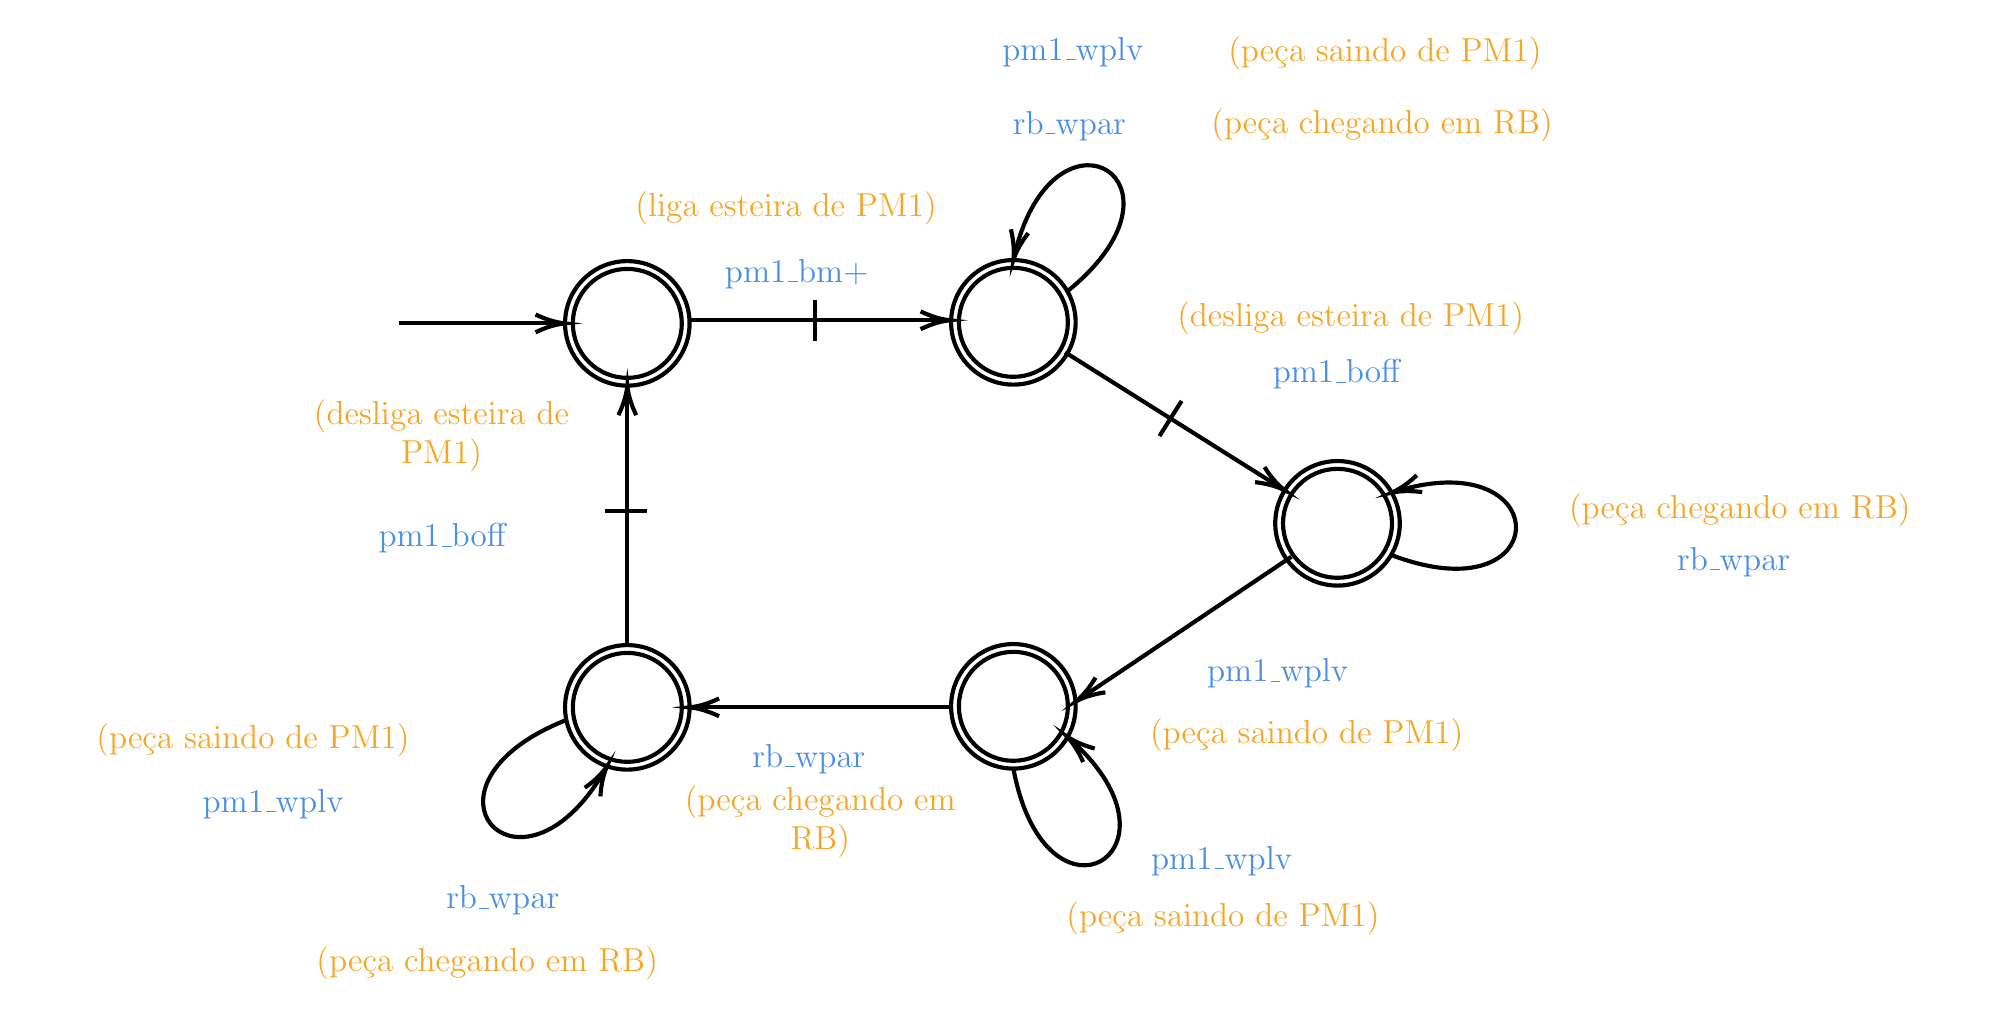
\begin{tikzpicture}[x=0.75pt,y=0.75pt,yscale=-1,xscale=1]
%uncomment if require: \path (0,3420); %set diagram left start at 0, and has height of 3420

%Shape: Circle [id:dp23601440540319296] 
\draw  [line width=1.5]  (1669.5,2181.5) .. controls (1669.5,2164.93) and (1682.93,2151.5) .. (1699.5,2151.5) .. controls (1716.07,2151.5) and (1729.5,2164.93) .. (1729.5,2181.5) .. controls (1729.5,2198.07) and (1716.07,2211.5) .. (1699.5,2211.5) .. controls (1682.93,2211.5) and (1669.5,2198.07) .. (1669.5,2181.5) -- cycle ;
%Shape: Circle [id:dp2022980675381547] 
\draw  [line width=1.5]  (1673.25,2181.5) .. controls (1673.25,2167) and (1685,2155.25) .. (1699.5,2155.25) .. controls (1714,2155.25) and (1725.75,2167) .. (1725.75,2181.5) .. controls (1725.75,2196) and (1714,2207.75) .. (1699.5,2207.75) .. controls (1685,2207.75) and (1673.25,2196) .. (1673.25,2181.5) -- cycle ;
%Straight Lines [id:da20360687176649162] 
\draw [line width=1.5]    (1589.5,2181.5) -- (1666.5,2181.5) ;
\draw [shift={(1669.5,2181.5)}, rotate = 180] [color={rgb, 255:red, 0; green, 0; blue, 0 }  ][line width=1.5]    (14.21,-4.28) .. controls (9.04,-1.82) and (4.3,-0.39) .. (0,0) .. controls (4.3,0.39) and (9.04,1.82) .. (14.21,4.28)   ;
%Shape: Circle [id:dp5581776719780993] 
\draw  [line width=1.5]  (1855.5,2181) .. controls (1855.5,2164.43) and (1868.93,2151) .. (1885.5,2151) .. controls (1902.07,2151) and (1915.5,2164.43) .. (1915.5,2181) .. controls (1915.5,2197.57) and (1902.07,2211) .. (1885.5,2211) .. controls (1868.93,2211) and (1855.5,2197.57) .. (1855.5,2181) -- cycle ;
%Straight Lines [id:da6469225581898377] 
\draw [line width=1.5]    (1910.42,2195.41) -- (1929.89,2207.65) -- (2013.71,2260.33) ;
\draw [shift={(2016.25,2261.93)}, rotate = 212.15] [color={rgb, 255:red, 0; green, 0; blue, 0 }  ][line width=1.5]    (14.21,-4.28) .. controls (9.04,-1.82) and (4.3,-0.39) .. (0,0) .. controls (4.3,0.39) and (9.04,1.82) .. (14.21,4.28)   ;
%Straight Lines [id:da9071024479041658] 
\draw [line width=1.5]    (1966.54,2218.87) -- (1955.9,2235.8) ;

%Shape: Circle [id:dp40872647102696935] 
\draw  [line width=1.5]  (1855.5,2366) .. controls (1855.5,2349.43) and (1868.93,2336) .. (1885.5,2336) .. controls (1902.07,2336) and (1915.5,2349.43) .. (1915.5,2366) .. controls (1915.5,2382.57) and (1902.07,2396) .. (1885.5,2396) .. controls (1868.93,2396) and (1855.5,2382.57) .. (1855.5,2366) -- cycle ;
%Shape: Circle [id:dp5565476487030998] 
\draw  [line width=1.5]  (1669.5,2366.5) .. controls (1669.5,2349.93) and (1682.93,2336.5) .. (1699.5,2336.5) .. controls (1716.07,2336.5) and (1729.5,2349.93) .. (1729.5,2366.5) .. controls (1729.5,2383.07) and (1716.07,2396.5) .. (1699.5,2396.5) .. controls (1682.93,2396.5) and (1669.5,2383.07) .. (1669.5,2366.5) -- cycle ;
%Straight Lines [id:da9239255372434181] 
\draw [line width=1.5]    (1854.5,2366.5) -- (1831.5,2366.5) -- (1732.5,2366.5) ;
\draw [shift={(1729.5,2366.5)}, rotate = 360] [color={rgb, 255:red, 0; green, 0; blue, 0 }  ][line width=1.5]    (14.21,-4.28) .. controls (9.04,-1.82) and (4.3,-0.39) .. (0,0) .. controls (4.3,0.39) and (9.04,1.82) .. (14.21,4.28)   ;
%Straight Lines [id:da8733738548126078] 
\draw [line width=1.5]    (1708.9,2272) -- (1688.9,2272) ;
%Shape: Boxed Line [id:dp4537179801660236] 
\draw [line width=1.5]    (1699.5,2336.5) -- (1699.5,2214.5) ;
\draw [shift={(1699.5,2211.5)}, rotate = 90] [color={rgb, 255:red, 0; green, 0; blue, 0 }  ][line width=1.5]    (14.21,-4.28) .. controls (9.04,-1.82) and (4.3,-0.39) .. (0,0) .. controls (4.3,0.39) and (9.04,1.82) .. (14.21,4.28)   ;
%Shape: Circle [id:dp4448293272065569] 
\draw  [line width=1.5]  (1859.25,2181) .. controls (1859.25,2166.5) and (1871,2154.75) .. (1885.5,2154.75) .. controls (1900,2154.75) and (1911.75,2166.5) .. (1911.75,2181) .. controls (1911.75,2195.5) and (1900,2207.25) .. (1885.5,2207.25) .. controls (1871,2207.25) and (1859.25,2195.5) .. (1859.25,2181) -- cycle ;
%Shape: Circle [id:dp7597357964705245] 
\draw  [line width=1.5]  (1673.25,2366.5) .. controls (1673.25,2352) and (1685,2340.25) .. (1699.5,2340.25) .. controls (1714,2340.25) and (1725.75,2352) .. (1725.75,2366.5) .. controls (1725.75,2381) and (1714,2392.75) .. (1699.5,2392.75) .. controls (1685,2392.75) and (1673.25,2381) .. (1673.25,2366.5) -- cycle ;
%Shape: Circle [id:dp8656429564666801] 
\draw  [line width=1.5]  (1859.25,2366) .. controls (1859.25,2351.5) and (1871,2339.75) .. (1885.5,2339.75) .. controls (1900,2339.75) and (1911.75,2351.5) .. (1911.75,2366) .. controls (1911.75,2380.5) and (1900,2392.25) .. (1885.5,2392.25) .. controls (1871,2392.25) and (1859.25,2380.5) .. (1859.25,2366) -- cycle ;
%Shape: Circle [id:dp3733710350679478] 
\draw  [line width=1.5]  (2011.67,2277.83) .. controls (2011.67,2261.26) and (2025.1,2247.83) .. (2041.67,2247.83) .. controls (2058.24,2247.83) and (2071.67,2261.26) .. (2071.67,2277.83) .. controls (2071.67,2294.4) and (2058.24,2307.83) .. (2041.67,2307.83) .. controls (2025.1,2307.83) and (2011.67,2294.4) .. (2011.67,2277.83) -- cycle ;
%Shape: Circle [id:dp8182020576096669] 
\draw  [line width=1.5]  (2015.42,2277.83) .. controls (2015.42,2263.34) and (2027.17,2251.58) .. (2041.67,2251.58) .. controls (2056.16,2251.58) and (2067.92,2263.34) .. (2067.92,2277.83) .. controls (2067.92,2292.33) and (2056.16,2304.08) .. (2041.67,2304.08) .. controls (2027.17,2304.08) and (2015.42,2292.33) .. (2015.42,2277.83) -- cycle ;
%Shape: Boxed Bezier Curve [id:dp5547457937556954] 
\draw [line width=1.5]    (1911.43,2166.1) .. controls (1972.82,2116.52) and (1914.13,2075.67) .. (1890.64,2133.93) .. controls (1888.94,2138.14) and (1887.42,2142.87) .. (1886.15,2148.15) ;
\draw [shift={(1885.5,2151)}, rotate = 282.21] [color={rgb, 255:red, 0; green, 0; blue, 0 }  ][line width=1.5]    (14.21,-4.28) .. controls (9.04,-1.82) and (4.3,-0.39) .. (0,0) .. controls (4.3,0.39) and (9.04,1.82) .. (14.21,4.28)   ;
%Shape: Boxed Line [id:dp33908331846833417] 
\draw [line width=1.5]    (2019.44,2293.94) -- (1918.15,2361.95) ;
\draw [shift={(1915.66,2363.62)}, rotate = 326.12] [color={rgb, 255:red, 0; green, 0; blue, 0 }  ][line width=1.5]    (14.21,-4.28) .. controls (9.04,-1.82) and (4.3,-0.39) .. (0,0) .. controls (4.3,0.39) and (9.04,1.82) .. (14.21,4.28)   ;
%Shape: Boxed Bezier Curve [id:dp3416016771200352] 
\draw [line width=1.5]    (2067.67,2293.11) .. controls (2141.4,2321.22) and (2147.18,2249.95) .. (2085,2258.96) .. controls (2080.51,2259.61) and (2075.66,2260.68) .. (2070.46,2262.24) ;
\draw [shift={(2067.67,2263.11)}, rotate = 342] [color={rgb, 255:red, 0; green, 0; blue, 0 }  ][line width=1.5]    (14.21,-4.28) .. controls (9.04,-1.82) and (4.3,-0.39) .. (0,0) .. controls (4.3,0.39) and (9.04,1.82) .. (14.21,4.28)   ;
%Shape: Boxed Bezier Curve [id:dp4418114948340497] 
\draw [line width=1.5]    (1885.5,2396) .. controls (1900.02,2473.56) and (1963.82,2441.28) .. (1923.68,2392.96) .. controls (1920.78,2389.47) and (1917.33,2385.89) .. (1913.29,2382.26) ;
\draw [shift={(1911.09,2380.34)}, rotate = 40.53] [color={rgb, 255:red, 0; green, 0; blue, 0 }  ][line width=1.5]    (14.21,-4.28) .. controls (9.04,-1.82) and (4.3,-0.39) .. (0,0) .. controls (4.3,0.39) and (9.04,1.82) .. (14.21,4.28)   ;
%Shape: Boxed Bezier Curve [id:dp3570860014303048] 
\draw [line width=1.5]    (1669.29,2372.91) .. controls (1596.13,2402.47) and (1640.38,2458.64) .. (1679.82,2409.74) .. controls (1682.67,2406.2) and (1685.49,2402.12) .. (1688.25,2397.43) ;
\draw [shift={(1689.7,2394.9)}, rotate = 119.13] [color={rgb, 255:red, 0; green, 0; blue, 0 }  ][line width=1.5]    (14.21,-4.28) .. controls (9.04,-1.82) and (4.3,-0.39) .. (0,0) .. controls (4.3,0.39) and (9.04,1.82) .. (14.21,4.28)   ;
%Straight Lines [id:da1195292766490681] 
\draw [line width=1.5]    (1730,2180) -- (1753,2180) -- (1852,2180) ;
\draw [shift={(1855,2180)}, rotate = 180] [color={rgb, 255:red, 0; green, 0; blue, 0 }  ][line width=1.5]    (14.21,-4.28) .. controls (9.04,-1.82) and (4.3,-0.39) .. (0,0) .. controls (4.3,0.39) and (9.04,1.82) .. (14.21,4.28)   ;
%Straight Lines [id:da8661652565645079] 
\draw [line width=1.5]    (1790,2170) -- (1790,2190) ;


% Text Node
\draw (1781.17,2157.83) node  [font=\large] [align=left] {\begin{minipage}[lt]{58.23pt}\setlength\topsep{0pt}
\begin{center}
\textcolor[rgb]{0.29,0.56,0.89}{pm1\_bm+}
\end{center}

\end{minipage}};
% Text Node
\draw (1776.01,2126) node  [font=\large] [align=left] {\begin{minipage}[lt]{119.21pt}\setlength\topsep{0pt}
\begin{center}
\textcolor[rgb]{0.96,0.65,0.14}{(liga esteira de PM1)}
\end{center}

\end{minipage}};
% Text Node
\draw (1787,2391.5) node  [font=\large] [align=left] {\begin{minipage}[lt]{57.55pt}\setlength\topsep{0pt}
\begin{center}
\textcolor[rgb]{0.29,0.56,0.89}{rb\_wpar}
\end{center}

\end{minipage}};
% Text Node
\draw (1792.5,2421.5) node  [font=\large] [align=left] {\begin{minipage}[lt]{112.65pt}\setlength\topsep{0pt}
\begin{center}
\textcolor[rgb]{0.96,0.65,0.14}{(peça chegando em RB)}
\end{center}

\end{minipage}};
% Text Node
\draw (1610.33,2285.17) node  [font=\large] [align=left] {\begin{minipage}[lt]{57.55pt}\setlength\topsep{0pt}
\begin{center}
\textcolor[rgb]{0.29,0.56,0.89}{pm1\_boff}
\end{center}

\end{minipage}};
% Text Node
\draw (1610,2235.5) node  [font=\large] [align=left] {\begin{minipage}[lt]{119.22pt}\setlength\topsep{0pt}
\begin{center}
\textcolor[rgb]{0.96,0.65,0.14}{(desliga esteira de PM1)}
\end{center}

\end{minipage}};
% Text Node
\draw (1914.17,2050.83) node  [font=\large] [align=left] {\begin{minipage}[lt]{58.23pt}\setlength\topsep{0pt}
\begin{center}
\textcolor[rgb]{0.29,0.56,0.89}{pm1\_wplv}
\end{center}

\end{minipage}};
% Text Node
\draw (2064.5,2051.5) node  [font=\large] [align=left] {\begin{minipage}[lt]{156.17pt}\setlength\topsep{0pt}
\begin{center}
\textcolor[rgb]{0.96,0.65,0.14}{(peça saindo de PM1)}
\end{center}

\end{minipage}};
% Text Node
\draw (1912.5,2086.5) node  [font=\large] [align=left] {\begin{minipage}[lt]{58.23pt}\setlength\topsep{0pt}
\begin{center}
\textcolor[rgb]{0.29,0.56,0.89}{rb\_wpar}
\end{center}

\end{minipage}};
% Text Node
\draw (2063.17,2085.83) node  [font=\large] [align=left] {\begin{minipage}[lt]{156.17pt}\setlength\topsep{0pt}
\begin{center}
\textcolor[rgb]{0.96,0.65,0.14}{(peça chegando em RB)}
\end{center}

\end{minipage}};
% Text Node
\draw (2041.17,2206.17) node  [font=\large] [align=left] {\begin{minipage}[lt]{58.23pt}\setlength\topsep{0pt}
\begin{center}
\textcolor[rgb]{0.29,0.56,0.89}{pm1\_boff}
\end{center}

\end{minipage}};
% Text Node
\draw (2048.01,2178.83) node  [font=\large] [align=left] {\begin{minipage}[lt]{143.25pt}\setlength\topsep{0pt}
\begin{center}
\textcolor[rgb]{0.96,0.65,0.14}{(desliga esteira de PM1)}
\end{center}

\end{minipage}};
% Text Node
\draw (2012.83,2350.17) node  [font=\large] [align=left] {\begin{minipage}[lt]{58.23pt}\setlength\topsep{0pt}
\begin{center}
\textcolor[rgb]{0.29,0.56,0.89}{pm1\_wplv}
\end{center}

\end{minipage}};
% Text Node
\draw (2026.83,2379.83) node  [font=\large] [align=left] {\begin{minipage}[lt]{156.17pt}\setlength\topsep{0pt}
\begin{center}
\textcolor[rgb]{0.96,0.65,0.14}{(peça saindo de PM1)}
\end{center}

\end{minipage}};
% Text Node
\draw (2232.5,2296.5) node  [font=\large] [align=left] {\begin{minipage}[lt]{58.23pt}\setlength\topsep{0pt}
\begin{center}
\textcolor[rgb]{0.29,0.56,0.89}{rb\_wpar}
\end{center}

\end{minipage}};
% Text Node
\draw (2235.5,2271.5) node  [font=\large] [align=left] {\begin{minipage}[lt]{156.17pt}\setlength\topsep{0pt}
\begin{center}
\textcolor[rgb]{0.96,0.65,0.14}{(peça chegando em RB)}
\end{center}

\end{minipage}};
% Text Node
\draw (1985.83,2440.5) node  [font=\large] [align=left] {\begin{minipage}[lt]{58.23pt}\setlength\topsep{0pt}
\begin{center}
\textcolor[rgb]{0.29,0.56,0.89}{pm1\_wplv}
\end{center}

\end{minipage}};
% Text Node
\draw (1986.5,2468.17) node  [font=\large] [align=left] {\begin{minipage}[lt]{156.17pt}\setlength\topsep{0pt}
\begin{center}
\textcolor[rgb]{0.96,0.65,0.14}{(peça saindo de PM1)}
\end{center}

\end{minipage}};
% Text Node
\draw (1528.83,2413.17) node  [font=\large] [align=left] {\begin{minipage}[lt]{58.23pt}\setlength\topsep{0pt}
\begin{center}
\textcolor[rgb]{0.29,0.56,0.89}{pm1\_wplv}
\end{center}

\end{minipage}};
% Text Node
\draw (1519.17,2382.5) node  [font=\large] [align=left] {\begin{minipage}[lt]{156.17pt}\setlength\topsep{0pt}
\begin{center}
\textcolor[rgb]{0.96,0.65,0.14}{(peça saindo de PM1)}
\end{center}

\end{minipage}};
% Text Node
\draw (1639.5,2459.5) node  [font=\large] [align=left] {\begin{minipage}[lt]{58.23pt}\setlength\topsep{0pt}
\begin{center}
\textcolor[rgb]{0.29,0.56,0.89}{rb\_wpar}
\end{center}

\end{minipage}};
% Text Node
\draw (1632,2490) node  [font=\large] [align=left] {\begin{minipage}[lt]{156.17pt}\setlength\topsep{0pt}
\begin{center}
\textcolor[rgb]{0.96,0.65,0.14}{(peça chegando em RB)}
\end{center}

\end{minipage}};


\end{tikzpicture}